\documentclass[9pt,notheorems]{beamer} %global font-size
\usepackage{UESTC}

\usepackage{hyperref}
\usepackage[T1]{fontenc}
\usepackage{latexsym,amsmath,xcolor,multicol,booktabs,calligra}
\usepackage{graphicx,pstricks,listings,stackengine}
\usepackage[linesnumbered,ruled,vlined]{algorithm2e}
\usepackage{multirow}
\usepackage{pgfpages}

\author{Zhengren Wang}
\title{Listing Maximal $k$-Plexes in Large Real-World Graphs}
\subtitle{Zhengren Wang, Yi Zhou, Mingyu Xiao, Bakhadyr Khoussainov}
\institute{Algorithms and Logic Group in UESTC}
\date{\today}

\begin{document}

\begin{frame}
    \titlepage
    \begin{figure}[htpb]
        \begin{center}
            
\includegraphics[width=0.2\linewidth]{pic/logo.pdf}
        \end{center}
    \end{figure}
\end{frame}

\begin{frame}
    \tableofcontents[sectionstyle=show,subsectionstyle=show/shaded/hide,subsubsectionstyle=show/shaded/hide]
\end{frame}

\section{Background}
\begin{frame}{Finding Cohesive Groups}
    \vspace{0.5cm}
    Finding \textbf{\emph{cohesive groups}} (or \textbf{\emph{communities}}) has received attention from various areas.
    \begin{itemize}
	    \item In the WWW, identify clients sharing similar interests and serve them with a common proxy to reduce network traffic.
	    \item In social networks, discover closely related individuals.
		\item In biological networks, predict the structure and function of protein.
	\end{itemize}
    \begin{figure}[h]
    \centering
    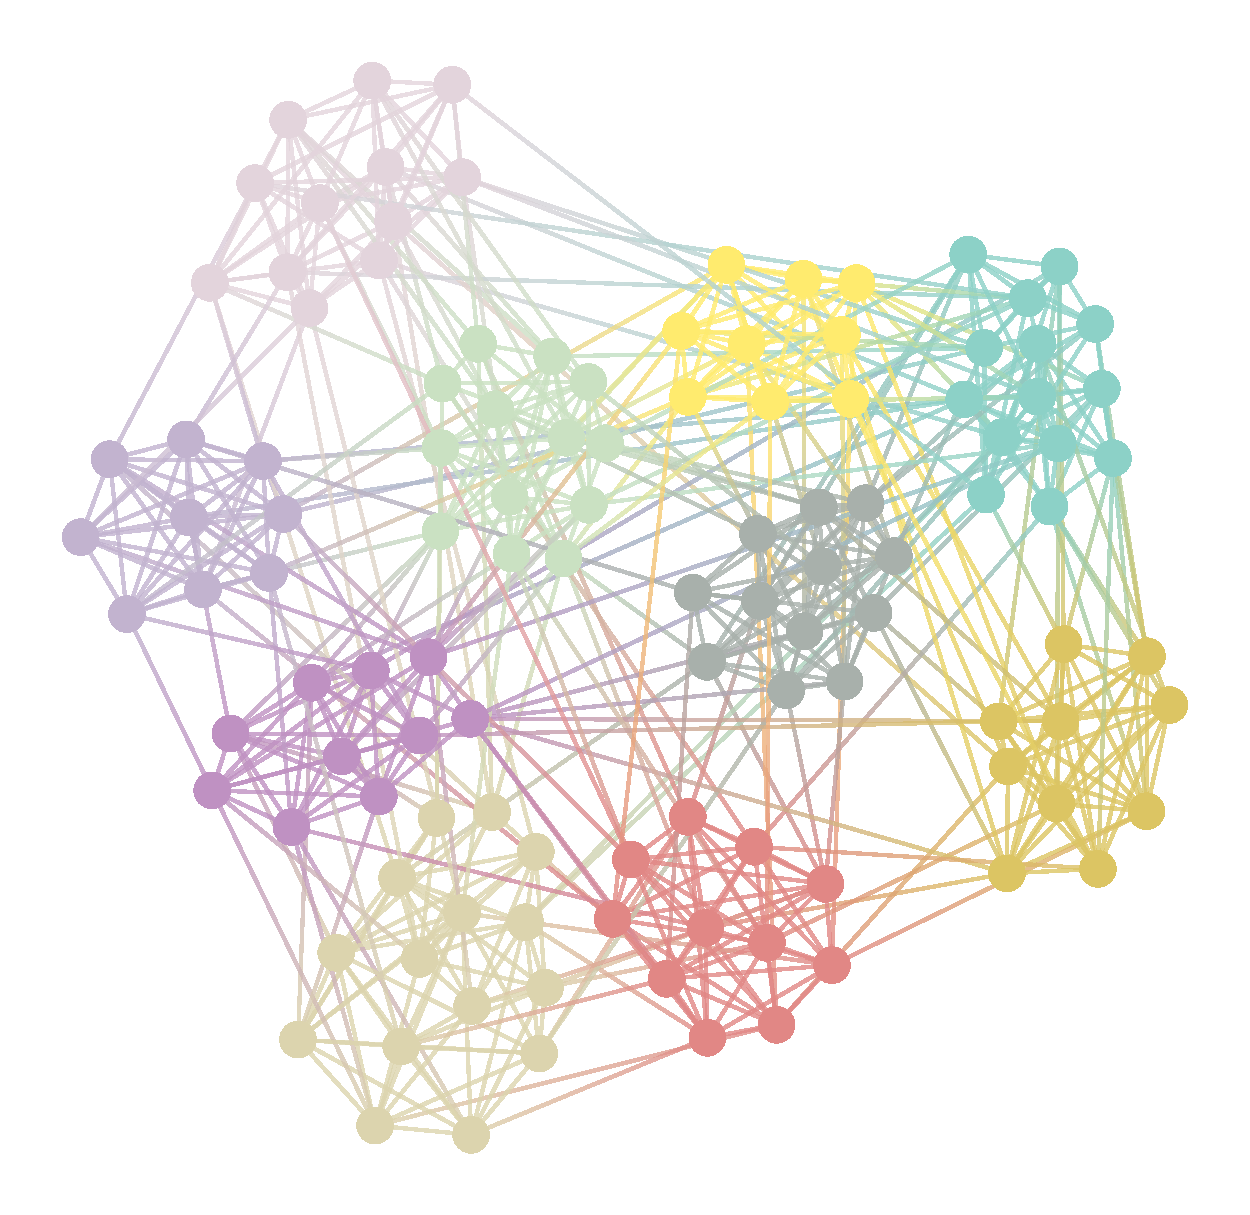
\includegraphics[width=0.4\linewidth]{pic/cohesive_groups.pdf}
    \end{figure}
\end{frame}
\begin{frame}{Clique Model}
    Naturally, cohesive groups can be modeled with \textbf{\emph{Cliques}}.
    
    A clique is a subgraph where vertices are pairwise connected, i.e., a complete graph.
    
    \centering
    \begin{minipage}[c]{0.4\linewidth}
        \psset{unit=0.8cm}
        \begin{figure}[h]
            \centering
            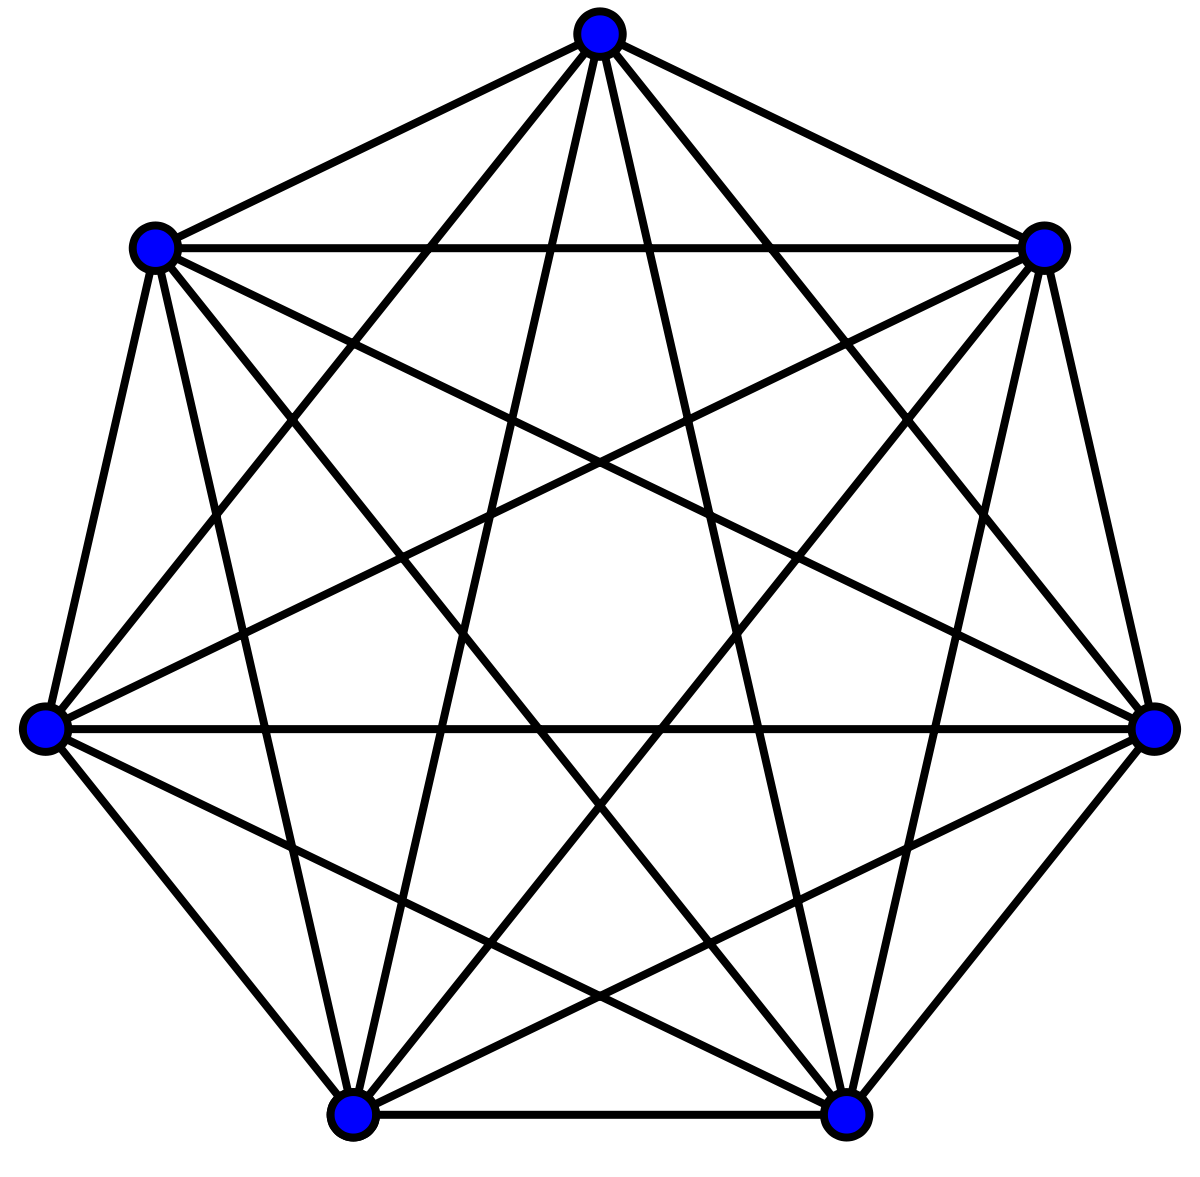
\includegraphics[height=.3\textheight]{pic/k7.png}\\
            \caption{$K_7$}
        \end{figure}
    \end{minipage}\hspace{1cm}
    \begin{minipage}{0.4\linewidth}
        \medskip
        %\hspace{2cm}
        \begin{figure}[h]
            \centering
            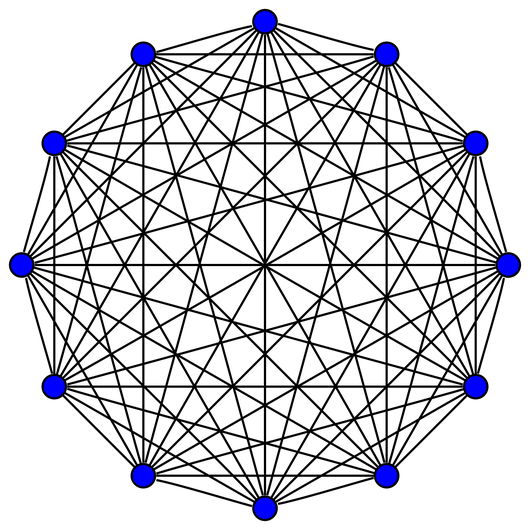
\includegraphics[height=.3\textheight]{pic/k12.png}\\
            \caption{$K_{12}$}
        \end{figure}
    \end{minipage}
\end{frame}
\begin{frame}{$k$-Plex Model}
    Due to various reasons like \emph{data noise}, communities rarely appear as cliques.
    
    \textbf{\emph{k-Plexes}} allow every vertex missing at most $k-1$ links to other vertices.

    \begin{figure}[h]
        \centering
        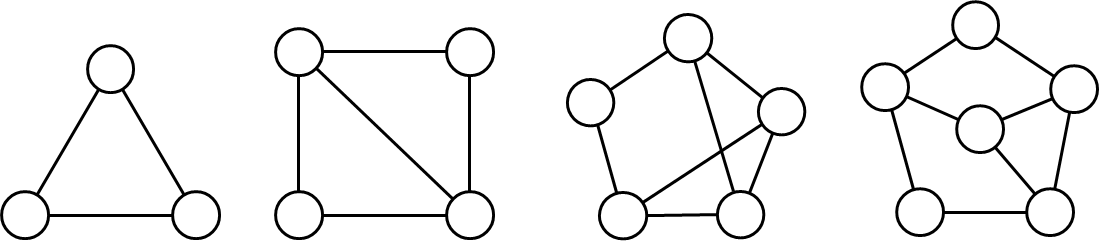
\includegraphics[width=0.8\linewidth]{pic/plexes.png}\\
        \caption{$1,2,3,4$-plex}
    \end{figure}
\end{frame}
\begin{frame}{Properties}
    \begin{lemma}[Hereditary Property]
        \begin{itemize}
            \item Any induced subgraph of a $k$-plex is still a $k$-plex.
            \item A $k$-plex is maximal if it is not a subgraph of any larger $k$-plex.
        \end{itemize}
    \end{lemma}
    \begin{lemma}[Distance Property]
        \begin{itemize}
            \item Any $k$-plex with at least $2k-1$ vertices has its diameter at most 2.
            \item A $k$-plex with at most $2k-2$ vertices may be unconnected.
        \end{itemize}
    \end{lemma}
    \begin{figure}[h]
        \centering
        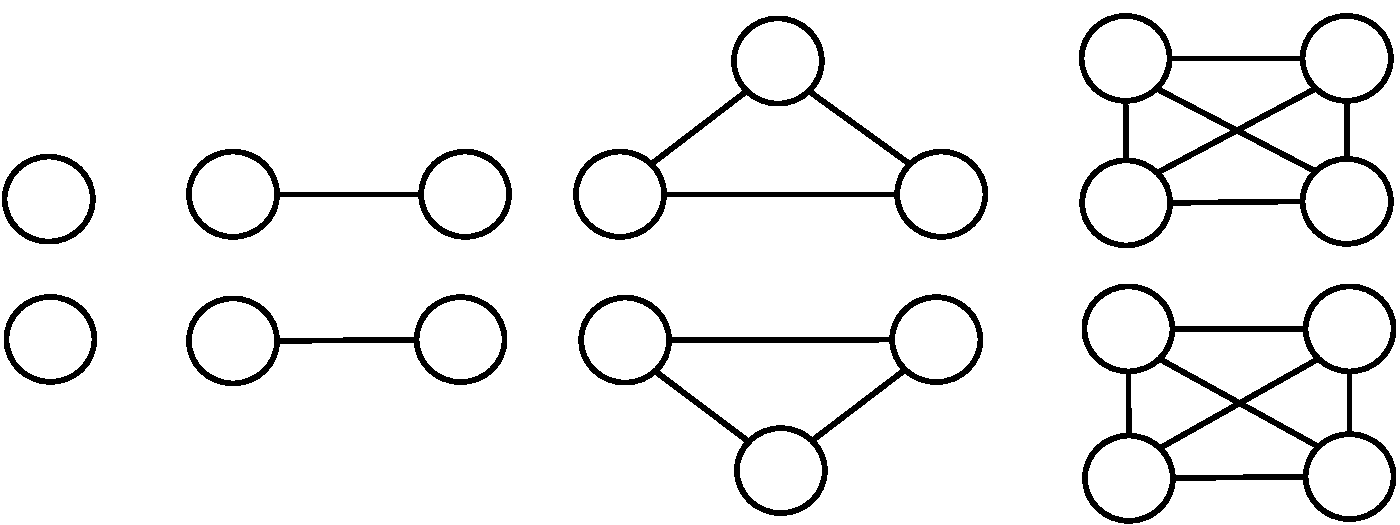
\includegraphics[width=0.5\linewidth]{pic/unconnected.pdf}\\
        \caption{unconnected $2,3,4,5$-plex}
    \end{figure}
\end{frame}
\begin{frame}{Translated Problems}
    We model cohesive groups with \textbf{\emph{maximal k-plexes}}.
    
    \begin{problem}[Listing maximal $k$-plexes]
        Given a graph $G$, a positive integer $k$, list all maximal $k$-plexes from $G$.
    \end{problem}
    \begin{problem}[Listing large maximal $k$-plexes]
        Given a graph $G$, two positive integers $k$ and $l$ where $l \ge 2k-1$, list all maximal $k$-plexes with at least $l$ vertices.
    \end{problem}

    % \pause
    % \vspace{0.5cm}
    % \begin{center}
    %     We propose \emph{ListPlex} to solve them.
    % \end{center}
\end{frame}
% \section{Primitive}
% \begin{frame}{Basic Definitions}
%     \begin{itemize} 
%         \item $N^k_G(v)$ is the set of vertices with distance exactly $k$ to $v$, say $k$-hop neighbors of $v$.
%         \item Given an ordering $\eta =v_1,. . .,v_n$ of $V$. 
%         \begin{itemize}
%             \item $N^k_{\prec_\eta}(v_i)$ is $N^k(v_i)\cap \{v_1,...,v_{i-1}\}$.
%             \item $N^k_{\succ_\eta}(v_i)$  is $N^k(v_i) \cap \{v_{i+1},...,v_n\}$.
%         \end{itemize}
%     \end{itemize}
% \end{frame}
\section{Algorithms}
\begin{frame}{The Bron-Kerbosch Algorithm}
    Our algorithm stems from the Bron-Kerbosch algorithm, say \emph{BKPlex}.\\
    BKPlex accepts three sets $P$, $C$ and $X$ as parameters,
    \begin{itemize}
        \item $P$: \textbf{\emph{plex vertices}} of the growing $k$-plex,
        \item $C$: \textbf{\emph{candidate vertices}} for further branching,
        \item $X$: \textbf{\emph{excluded vertices}} to avoid non-maximal solutions.
    \end{itemize}
    then lists maximal $k$-plexes $G[P']$ with three properties: \\
    \begin{minipage}{0.14\linewidth}
        \begin{itemize}
            \item $P \subseteq P'$
        \end{itemize}
    \end{minipage}
    \begin{minipage}{0.18\linewidth}
        \begin{itemize}
            \item $P' \subseteq P\cup C$
        \end{itemize}
    \end{minipage}
    \begin{minipage}{0.65\linewidth}
        \begin{itemize}
            \item $\forall v\in X$, the subgraph $G[\{v\} \cup P']$ is not a $k$-plex.
        \end{itemize}
    \end{minipage}\\
    \vspace{0.25cm}
    \begin{flushright}
        \footnotesize \textbf{\emph{Hereditary Prop.}} Any induced subgraph of a $k$-plex is still a $k$-plex.
    \end{flushright}
\end{frame}
\begin{frame}{The Bron-Kerbosch Algorithm}
    \begin{center}
        BKPlex branches by doing bipartition recursively. \footnote{Simplified for clarity. In fact, a variant of bipartition.}
    \end{center}
    \begin{figure}
    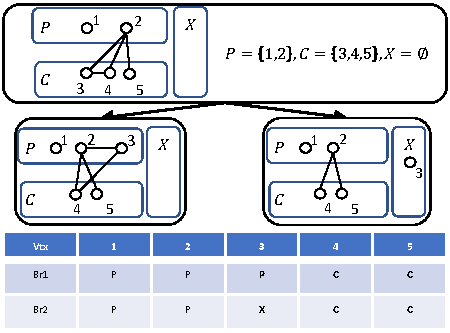
\includegraphics[width=0.65\linewidth]{pic/bkrec.pdf}\\
    \caption{An example of BKPlex.}
\end{figure}
\end{frame}
\begin{frame}{Degeneracy Ordering}
    \begin{itemize}
        \item $\eta =v_1,. . .,v_n$ is called \emph{degeneracy ordering} (\emph{core ordering}) if each vertex $v_i$ has the minimum degree in the induced subgraph $G[\{v_i,...,v_n\}]$.
        \item Given a degeneracy ordering $\eta =v_1,. . .,v_n$, the degree of $v_i$ in $G[\{v_i,...,v_n\}]$ is called the \emph{core number} of $v_i$. 
        \item For any degeneracy ordering of the same graph, the largest core number among all vertices is a constant $D$ called \emph{degeneracy}.
        \item Due to the sparsity of many real-world graphs, $D \ll \Delta \ll n$ where $\Delta$ is the maximum degree.
    \end{itemize}
    \begin{figure}
        \only<1>{
            \begin{center}
                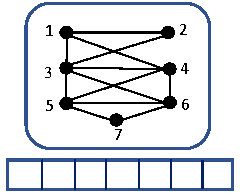
\includegraphics[width=0.3\linewidth]{pic/order_1.pdf}
            \end{center}
        }
        \only<2>{
            \begin{center}
                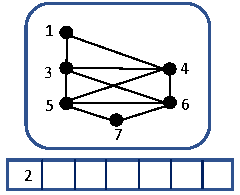
\includegraphics[width=0.3\linewidth]{pic/order_2.pdf}
            \end{center}
        }
        \only<3>{
            \begin{center}
                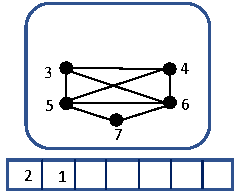
\includegraphics[width=0.3\linewidth]{pic/order_3.pdf}
            \end{center}
        }
        \only<4>{
            \begin{center}
                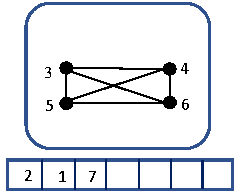
\includegraphics[width=0.3\linewidth]{pic/order_4.pdf}
            \end{center}
        }
        \only<5>{
            \begin{center}
                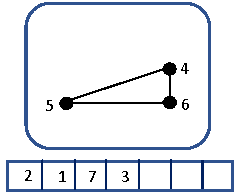
\includegraphics[width=0.3\linewidth]{pic/order_5.pdf}
            \end{center}
        }
        \only<6>{
            \begin{center}
                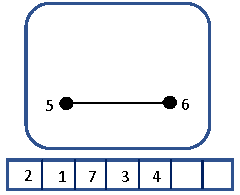
\includegraphics[width=0.3\linewidth]{pic/order_6.pdf}
            \end{center}
        }
        \only<7>{
            \begin{center}
                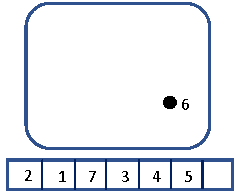
\includegraphics[width=0.3\linewidth]{pic/order_7.pdf}
            \end{center}
        }
        \only<8>{
            \begin{center}
                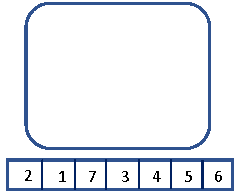
\includegraphics[width=0.3\linewidth]{pic/order_8.pdf}
            \end{center}
        }
        \only<9>{
            \begin{center}
                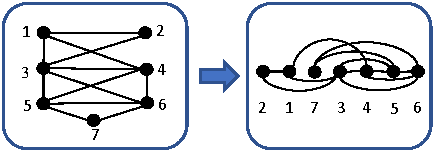
\includegraphics[width=0.6\linewidth]{pic/order.pdf}
            \end{center}
        }
        \caption{An example of degeneracy ordering.}
    \end{figure}
\end{frame}
\begin{frame}{Recent Algorithms  \footnote{Simplified for clarity.}}
    \textbf{\emph{Pivot Heuristic}} Zhou et al. (2020) proposed \emph{BKPivot} with a \emph{pivot} heuristic in the branch scheme of BKPlex, and improved its running time from $O^*(2^n)$ to $O^*(\gamma_k^n)$, where $\gamma_k<2$. \footnote{The notation $O^*$ omits the polynomial factors.}\\
    \vspace{0.5cm}    
    \textbf{\emph{Graph Decomposition}} Conte et al. (2018) proposed \emph{D2K}, a decomposition-based algorithm for listing $k$-plexes with the diameter at most 2.\\
    For each vertex, D2K builds a local subgraph and then adopts BKPlex to list maximal $k$-plexes locally which runs in $O^*(2^{D\Delta})$.\\
    \vspace{0.25cm}
    \begin{flushright}
        \footnotesize \textbf{\emph{Distance Prop.}} Any $k$-plex with at least $2k-1$ vertices has the diameter at most 2.
    \end{flushright}
    \pause
    \vspace{0.5cm}
    \begin{center}
        We combine them and propose \emph{ListPlex} running in $O^*(\gamma_k^D)$.
    \end{center}
\end{frame}
\begin{frame}{ListPlex}
    \framesubtitle{Listing All Maximal $k$-Plexes}
    Based on Distance Property, ListPlex divides its task into two parts.
    \begin{itemize}
        \item \emph{Part I}: k-plexes with size at most $2k-2$. \footnotesize (Solved directly by BKPlex) \normalsize
        \item \emph{\textbf{Part II}}: k-plexes with size at least $2k-1$.
    \end{itemize}
    \vspace{0.25cm}
    \begin{flushright}
        \footnotesize \textbf{\emph{Distance Prop.}} Any $k$-plex with at least $2k-1$ vertices has the diameter at most 2.
    \end{flushright}    
    % \vspace{0.5cm}
    % \begin{theorem}
    %     Given a graph $G$ with degeneracy $D$, for fixed $k$, ListPlex runs in $O^*(\gamma_k^D)$.
    % \end{theorem}
\end{frame}
\begin{frame}{ListPlex}
    \framesubtitle{Part II}
    \textbf{\emph{Procedure}}\\
    \vspace{0.25cm}
    1) Sort $V$ by a degeneracy ordering $\eta=v_1\dots v_n$.\\
    \begin{itemize}
        \item $N^k(v)$ denotes $k$-hop neighbors of $v$.
        \item $N^k_{\succ}(v_i)$ denotes $N^k(v_i) \cap \{v_{i+1},...,v_n\}$, say \textbf{\emph{forward}} $k$-hop neighbors of $v_i$
    \end{itemize}
    \vspace{0.2cm}
    2) From $v_1$ to $v_n$, in the $i$-th iteration, list maximal $k$-plexes with $i$ as the minimum index of vertices.
    \begin{itemize}
        \item Build \textbf{\emph{seed graph}} $G_i= G[\{v_i\}\cup  N_{\succ}(v_i) \cup N^2_{\succ}(v_i)]$.
        \item Call BKPivot with given combinations of $N^2_{\succ}(v_i)$, say \textbf{\emph{seed set}} $S$.
        \item Validate maximality in $G$ for $k$-plexes generated in $G_i$. 
    \end{itemize}
\end{frame}
\begin{frame}{ListPlex}
    \framesubtitle{Part II}
    \begin{figure}
        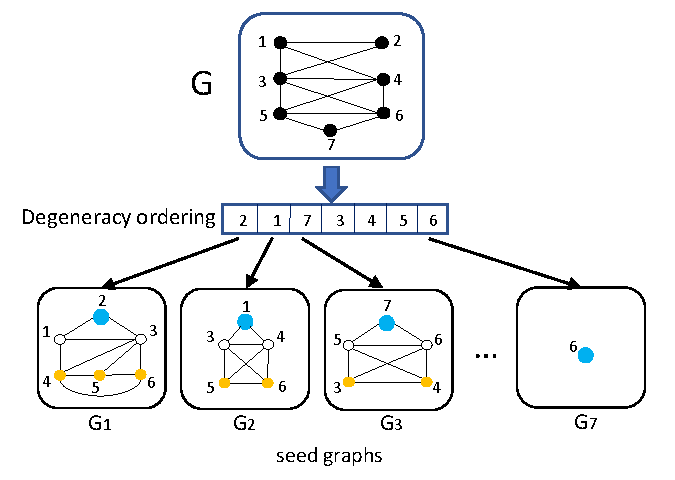
\includegraphics[width=0.49\linewidth]{pic/degen.pdf}
        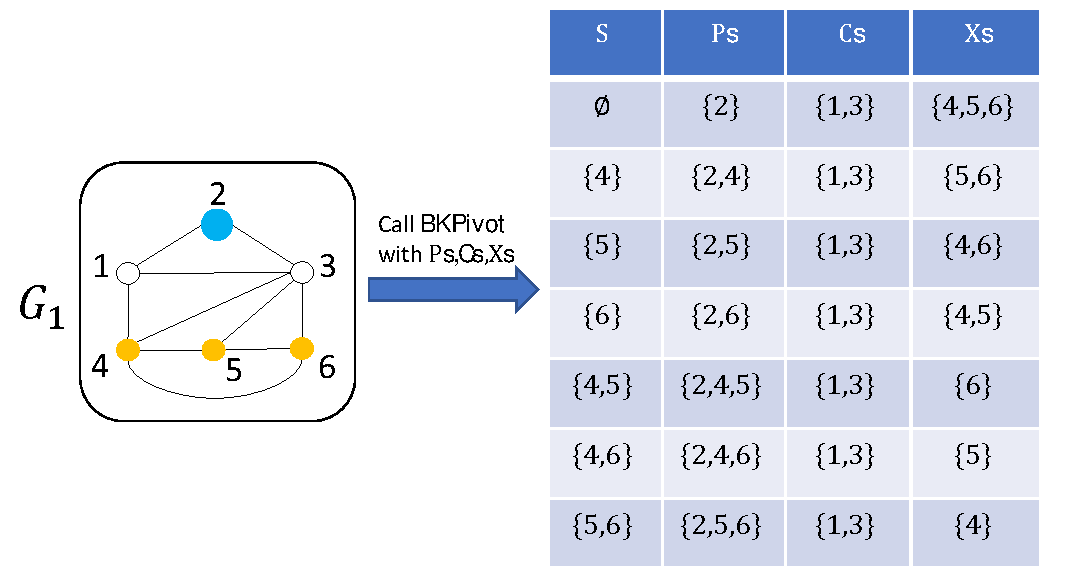
\includegraphics[width=0.49\linewidth]{pic/seeds.pdf}
        \caption{An example of ListPlex's Part II.

        (L) sort $V$ in degeneracy ordering $\eta$ and induce seed graphs $G_i$ for each $v_i \in \eta$.
        
        (R) enumerate $S\subseteq N^2_{\succ}(v_i)$ with bound $|S|\le k-1\;(k=3)$ and call BKPivot with $P_s, C_s, X_s$.
        }
    \end{figure}
\end{frame}
\begin{frame}{ListPlex}
    \framesubtitle{Graph Decompostion}
    \centering
    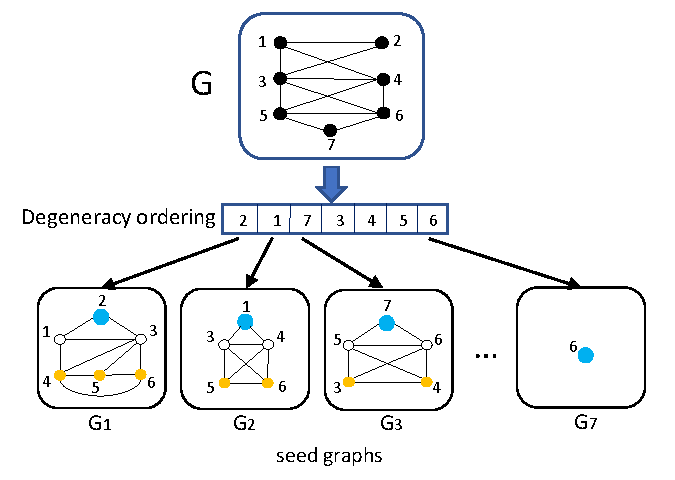
\includegraphics[width=0.7\linewidth]{pic/degen.pdf}\\
    \begin{minipage}{0.45\linewidth}
        \begin{itemize}
            \item Cohesive groups appear locally in large real-world graphs,
            \item Parallelism,
        \end{itemize}
    \end{minipage}     
    \begin{minipage}{0.45\linewidth}
        \begin{itemize}
            \item Smaller scale and better locality,
            \item $D \ll \Delta$.
        \end{itemize}
    \end{minipage}
\end{frame}
\begin{frame}{ListPlex}
    \framesubtitle{Seed Set}
    \centering
    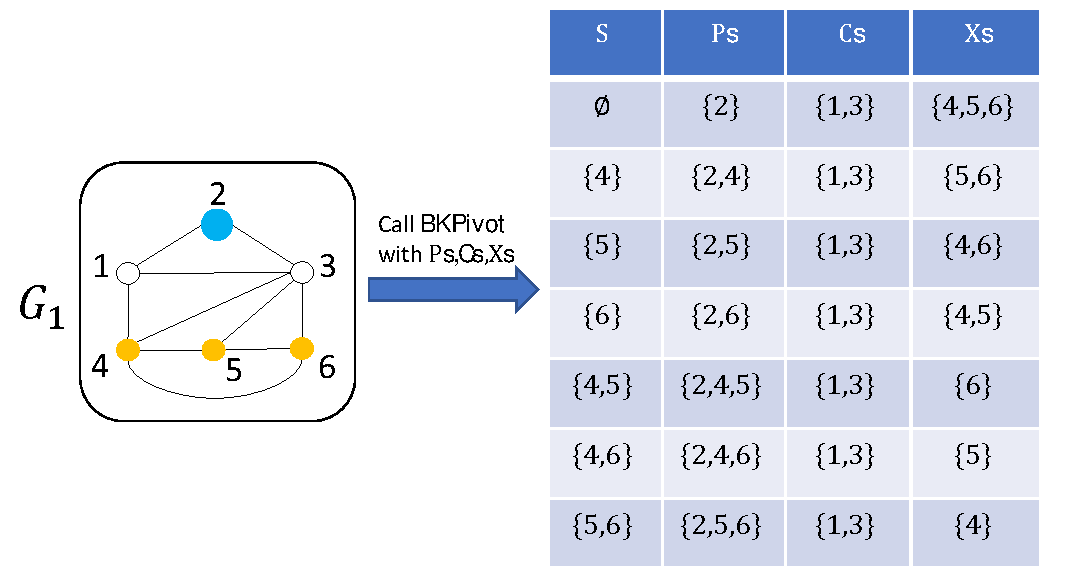
\includegraphics[width=0.8\linewidth]{pic/seeds.pdf}
    \begin{minipage}{0.45\linewidth}
        \begin{itemize}
            \item At most $k-1$ vertices come from $N^2_{\succ}(v_i)$,
            \item Reducing candidates fast,
        \end{itemize}
    \end{minipage}
    \begin{minipage}{0.45\linewidth}
        \begin{itemize}
            \item $|N^2_{\succ}(v_i)|$ is potentially $D\Delta$,
            \item Pruning rules.
        \end{itemize}
    \end{minipage}
\end{frame}
\begin{frame}{ListPlex}
    \framesubtitle{Listing Large Maximal k-Plexes}
    With lower bound $l$, a related lower bound $l'$ can be derived.
    \begin{lemma}
        Assume $|P|\ge l$, for any vertex pair $u,v \in P$,  $|N(u)\cap N(v) \cap P| \ge l'$
    \end{lemma}
    \vspace{0.25cm}
    Removing unfruitful candidates from $G_i$ reduces the scale of $G_i$.\\
    \begin{itemize}
        \item Consider vertex pair $(v_i,u)$, $u \in V_i$.
    \end{itemize}    
    \vspace{0.25cm}
    Dropping unfruitful seed sets $S$ saves the forthcoming exponential search.
    \begin{itemize}
        \item Consider vertex pair $(u,v)$ from some $S$.
    \end{itemize}       
\end{frame}
\section{Implementation Techniques}
\begin{frame}{Reducing cache misses}
    Validating maximality in $G$ for maximal $k$-plex of $G_i$ suffers a high amount of cache misses.\\
    \vspace{0.5cm}
    Alleviation:\\
    \begin{itemize}
    \item Build a bipartite graph $B_i$ for each $G_i$, which serves as a cache of currently useful data of large $G$,
    \item Pruning bipartite graph just like seed graph.
    \end{itemize}
\end{frame}
\begin{frame}{Parallelization}
    ListPlex owns appealing parallel features.\\
    \vspace{0.5cm}
    How To:\\
    \begin{itemize}
        \item Parallelize searches of maximal $k$-plexes on each $G_i$, say $T_i$,
        \item Split $T_i$ when some cores are idle for better load balance,
        \item Construct degeneracy ordering and perform generated $T_i$ in parallel. 
    \end{itemize}
\end{frame}
\section{Experiments}
\begin{frame}{Dataset}
    \centering
    All graphs are taken from SNAP and LAW \footnote{http://law.di.unimi.it/}.
    \begin{table}[h]
        % \scriptsize
        \centering
          \caption{Considered networks and their properties}
          \label{tbl-data}
          \resizebox{0.45\columnwidth}{!}{
              \begin{tabular}{c|c|c|c|c}
                \toprule[2pt]
                Network & n & m & $\Delta$ & D \\
                \hline
                jazz & 198 & 2742 & 100 & 29 \\
                ca-grqc & 5241 & 14484 & 81 & 43\\
                gnutella08 & 6301 & 41554 & 97 & 10\\
                wiki-vote & 7116 & 100763 & 1065 & 53\\
                lastfm & 7624 & 55612 & 216 & 20\\
                \hline
                as-caida & 26475 & 53381 & 2628 & 22\\
                soc-epinions & 75888 & 405739 & 3044 & 67\\
                soc-slashdot & 82144 & 500480 & 2548 & 54\\
                email-euall & 265214 & 365569 & 7636 & 37\\
                amazon0505 & 410236 & 2439436 & 2760 & 10\\
                in-2004 & 1353703 & 13126172 & 21869 & 488\\
                soc-pokec & 1632803 & 22301964 & 14854 & 47\\
                as-skitter & 1696415 & 11095298 & 35455 & 111\\
                soc-livejournal & 4847571 & 68993773 & 14815 & 360\\
                \hline
                arabic-2005 & 22744080 & 639999458 & 575628 & 3247\\
                uk-2005 & 39459925 & 936364282 & 1372171 & 584\\
                it-2004 & 41291594 & 1150725436 & 1243927 & 3209\\
                webbase-2001 & 118142155 & 1019903190 & 816127 & 1506\\
                \bottomrule[2pt]
        \end{tabular}
        }
        \end{table}
\end{frame}
\begin{frame}{Listing All Maximal $k$-Plexes}
    \begin{table}[h]
        \centering
          \caption{Listing all maximal $k$-plexes in small graphs}
          \label{tbl-pro1}
           \resizebox{0.8\linewidth}{!}{
            \begin{tabular}{c|c|c|c|c|c|c|c}
            \toprule[2pt]
            \multirow{2}{*}{Network} & \multirow{2}{*}{$k$} & \multirow{2}{*}{\#$k$-plexes} & \multicolumn{4}{c|}{The running time (s)} & \multirow{2}{*}{Speedup}\\
            \cline{4-7}
            & & & BKPlex & BKPivot & ListPlex & ListPlex(16)&\\
            \hline
            jazz  & 2     & 35214 & 648.864 & 0.29 & \textbf{0.086} & 0.408 & 0.211 \\
            jazz  & 3     & 3602575 & 772.826 & 17.55 & \textbf{6.477} & 0.832 & 7.785 \\
            jazz  & 4     & 193056583 & 3226.746 & 829.40 & \textbf{417.646} & 26.187 & 15.949 \\
            \hline
            ca-grqc & 2 & 13718439 & OOT & 1858.02 & \textbf{649.985} & 40.880 & 15.899\\
            \hline
            gnutella08 & 2 & 19866959 & 1500.208 & 3627.57 & \textbf{1117.858} & 70.207 & 15.922\\
            \hline
            wiki-vote & 2 & 66193264 & 10356.553 & 10671.92 & \textbf{1526.884} & 95.656 & 15.962\\
            \hline
            lastfm & 2 & 29086855 & 2643.394 & 6676.89 & \textbf{1989.701} & 124.525 & 15.978\\
            \bottomrule[2pt]
            \end{tabular}
            }
    \end{table}
\end{frame}
\begin{frame}{Listing Large Maximal $k$-Plexes}
    \begin{table}[t]
        \centering
        \caption{The running time of listing large maximal $k$-plexes from small and medium graphs by CommuPlex\footnotemark[5], D2K\footnotemark[6] and ListPlex.}
        \footnotetext[5]{Zhou et al. (2020)}
        \footnotetext[6]{Conte et al. (2018)}
        \label{tbl-community1}
        \resizebox{\linewidth}{!}{
        \begin{tabular}{c|c|c|c|c|c|c|c|c|c|c|c|c|c}
        \toprule[2pt]
        \multirow{2}{*}{\tabincell{c}{Graph\\ $(|V|,|E|)$}} & \multirow{2}{*}{$k$}    & \multirow{2}{*}{$l$} & \multirow{2}{*}{\#$k$-plexes}  &  \multicolumn{3}{c|}{The running time (s)}   & \multirow{2}{*}{\tabincell{c}{Graph\\ $(|V|,|E|)$}} & \multirow{2}{*}{$k$}    & \multirow{2}{*}{$l$} & \multirow{2}{*}{\#$k$-plexes}  &  \multicolumn{3}{c}{The running time (s)}
        \\
        \cline{5-7} \cline{12-14}
        & & & & CommuPlex & D2K & ListPlex & & & & & CommuPlex & D2K & ListPlex\\
        \hline
        
        \tabincell{c}{jazz (198, 2742)}
        & 4 & 12 & 2745953 & 25.218 & 33.054 & \textbf{4.498} &\multirow{9}{*}{\tabincell{c}{wiki-vote\\ (7116, 100763)}} & \multirow{3}{*}{2} & 12 & 2919931 & 75.871 & 115.757  & \textbf{17.653}  \\
        \cline{1-7}
        \tabincell{c}{lastfm (7624, 55612)} & 4 & 12 & 1827337 & 20.724 & 23.991 & \textbf{4.586} &  &  & 20 & 52 & 4.52 & 11.289 & \textbf{0.591} \\
        \cline{1-7}
        \multirow{2}{*}{\tabincell{c}{as-caida\\(26475, 53381)}} & 3 & 12 & 281251 & 5.684 & 13.421 & \textbf{0.867} & & & 30 & 0 & 1.033 & \textbf{0.027} & 0.091 \\
        \cline{2-7}  \cline{9-14}
         & 4 & 12 & 15939891 & 300.388 & 785.506 & \textbf{47.98} & & \multirow{3}{*}{3} & 12 & 458153397 & OOT & OOT & \textbf{2185.598} \\
        \cline{1-7}
        \multirow{3}{*}{\tabincell{c}{amazon0505\\(410236, 2439436)}} & 2 & 12 & 376 & 1.825 & 0.641 & \textbf{0.137} & & & 20 & 156727 & 595.636 & 1852.186 & \textbf{9.384} \\
        \cline{2-7}  & 3 & 12 & 6347 & 11.359 & 0.77  & \textbf{0.286} & & & 30 & 0 & 1.072 & \textbf{0.029} & 0.1 \\
        \cline{2-7} \cline{9-14} & 4 & 12 & 105649 & 47.049 & 5.338 & \textbf{1.171} & & \multirow{2}{*}{4} & 20 & 46729532 & OOT & OOT & \textbf{1174.2} \\
        \cline{1-7}   \multirow{4}{*}{\tabincell{c}{email-euall\\(265214, 365569)}} & 2 & 12 & 412779 & 8.793 & 11.199 & \textbf{1.946} & & & 30 & 0 & 9.17 & 3.627 & \textbf{0.112} \\
        \cline{2-14} & \multirow{2}{*}{3} & 12 & 32639016 & 619.384 & 1043.266 & \textbf{91.62} & \multirow{8}{*}{\tabincell{c}{soc-pokec\\(1632803, 22301964)}} & \multirow{3}{*}{2} & 12 & 7679906 & 1537.506 & 172.987 & \textbf{47.475} \\
        & & 20 & 2637 & 10.754 & 53.691 & \textbf{0.429} & & & 20 & 94184 & 1064.371 & 20.03 & \textbf{15.161} \\
        \cline{2-7} & 4 & 20 & 1707177 & 825.126 & 3800.889 & \textbf{24.089} & & & 30 & 3 & 662.64 & \textbf{8.637} & 9.557 \\
        \cline{1-7} \cline{9-14} \multirow{7}{*}{\tabincell{c}{soc-slashdot\\(82144, 500480)}} & \multirow{3}{*}{2} & 12 & 27208777 & 376.071 & 213.141 & \textbf{59.42} & & \multirow{3}{*}{3} & 12 & 520888893 & OOT & OOT & \textbf{1607.285} \\
        & & 20 & 11411028 & 227.016 & 137.159 & \textbf{32.988} & & & 20 & 5911456 & 1470.536 & 856.393 & \textbf{46.262} \\
        & & 30 & 453 & 10.77 & 16.481 & \textbf{0.688} & & & 30 & 5 & 717.425 & \textbf{9.993} & 10.127 \\
        \cline{2-7} \cline{9-14} & \multirow{3}{*}{3} & 12 & 2807943240 & OOT & 26029.006 & \textbf{7813.045} & & \multirow{2}{*}{4} & 20 & 318035938 & 34048.155 & OOT & \textbf{1825.216} \\
        & & 20 & 1303148522 & 28361.707 & 15308.777 & \textbf{4538.022} & & & 30 & 4515 & 1140.117 & 111.987 & \textbf{11.211} \\
        \cline{8-14} & & 30 & 1679468 & 699.876 & 2066.598 & \textbf{51.364} & \multirow{6}{*}{\tabincell{c}{soc-epinions\\(75888, 405739)}} & \multirow{3}{*}{2} & 12 & 49823056 & 843.9 & 735.589 & \textbf{193.307} \\
        \cline{2-7} & 4 & 30 & 502699966 & OOT & OOT & \textbf{6680.261} & & & 20 & 3322167 & 137.427 & 180.061 & \textbf{19.382} \\
        \cline{1-7} \multirow{4}{*}{\tabincell{c}{as-skitter\\(1696415, 11095298)}} & 2 & 50 & 47969775 & OOT & OOT & \textbf{520.884} & & & 30 & 0 & 8.995 & 12.109 & \textbf{0.492} \\
        \cline{9-14} & 2 & 100 & 0 & 1.793 & 2.951 & \textbf{0.716} & & \multirow{2}{*}{3} & 20 & 548634119 & 27037.614 & 35525.693 & \textbf{3072.267} \\
        \cline{2-7} & 3 & 50 & 21070497438 & OOT & OOT & OOT & & & 30 & 16066 & 546.69 & 2591.439 & \textbf{6.123} \\
        \cline{9-14} & 3 & 100 & 0 & 2.37 & 3.285 & \textbf{0.718} & & 4 & 30 & 13172906 & OOT & OOT & \textbf{661.103} \\
        \cline{1-7} \cline{8-14} \multirow{4}{*}{\tabincell{c}{in-2004\\(1353703, 13126172)}} & 2 & 50 & 25855779 & 7663.843 & 576.06 & \textbf{150.212} &\multirow{4}{*}{\tabincell{c}{com-livejournal\\(4847571, 68993773)}} & 2 & 340 & 650322 & 2284.435 & OOT & \textbf{109.382} \\
        & 2 & 100 & 9978037 & 5899.638 & 256.225 & \textbf{72.063} & & 2 & 345 & 0 & 57.548 & 13589.487 & \textbf{6.914} \\
        \cline{2-7} \cline{9-14} & 3 & 50 & 29045783792 & OOT & OOT & OOT & & 3 & 340 & 555718694 & OOT & OOT & \textbf{22863.467} \\
        & 3 & 100 & 4257410159 & OOT & OOT & \textbf{28384.76} & & 3 & 345 & 3963139 & 24861.871 & OOT & \textbf{826.183} \\
        \bottomrule[2pt]
        \end{tabular}
        }
    \end{table}
\end{frame}
\begin{frame}{Listing Large Maximal $k$-Plexes}
    \begin{minipage}{0.45\linewidth}
        \begin{table}[H]
            \centering
            \caption{The parallel running time of large networks by ListPlex and D2K with 16 threads.}
            \label{tbl-community2}
            \resizebox{\linewidth}{!}{
            \begin{tabular}{c|c|c|c|c|c}
            \toprule[2pt]
            \multirow{2}{*}{\tabincell{c}{Graph\\ $(|V|,|E|)$}} & \multirow{2}{*}{$k$}    & \multirow{2}{*}{$l$} & \multirow{2}{*}{\#$k$-plexes}  &  \multicolumn{2}{c}{The running time (s)}
            \\
            \cline{5-6}
            & & & & D2K(16) & ListPlex(16)\\
            \hline \multirow{4}{*}{\tabincell{c}{arabic-2005\\(22744080, 639999458)}} & 2 & 800 & 224870903 & 2195.272 & \textbf{714.159}\\
            & 2 & 1000  & 236897 & 151.328 & \textbf{40.202}\\
            \cline{2-6}
            & 3 & 800 & $>$25062182205 & OOT & OOT\\
            & 3 & 1000 & 34155502 & 587.967 & \textbf{128.737}\\
            \hline \multirow{4}{*}{\tabincell{c}{uk-2005\\(39459925, 936364282)}} & 2 & 250 & 106243475 & OOT & \textbf{355.855}\\
            & 2 & 500 & 256406 & 318.118 & \textbf{35.001}\\
            \cline{2-6}
            & 3 & 250 & $>$18336111409 & OOT & OOT\\
            & 3 & 500 & 28199814 & 9506.661 & \textbf{121.726}\\
            \hline \multirow{4}{*}{\tabincell{c}{it-2004\\(41291594, 1150725436)}} & 2 & 2000 & 675111 & 340.904 & \textbf{41.983} \\
            & 2 & 3000 & 675111 & 307.735 & \textbf{38.468} \\
            \cline{2-6}
            & 3 & 2000 & 197679229 & 4254.456 & \textbf{724.979}\\
            & 3 & 3000  & 197679229 & 4235.389 & \textbf{715.002} \\
            \hline \multirow{4}{*}{\tabincell{c}{webbase-2001\\(118142155,  1019903190)}} & 2 & 800 & 1599005 & 374.134 & \textbf{54.19} \\
            & 2 & 1000 & 1164383 & 346.393 & \textbf{53.651} \\
            \cline{2-6}
            & 3 & 800 & 1785341050 & 36116.817 &\textbf{5521.386} \\
            & 3 & 1000 & 1484341137 & 35005.343 & \textbf{6960.816} \\
            \bottomrule[2pt]
            \end{tabular}
            }
        \end{table}
    \end{minipage}\hspace{0.5cm}
    \begin{minipage}{0.45\linewidth}
        \begin{figure}[H]
            \centering
            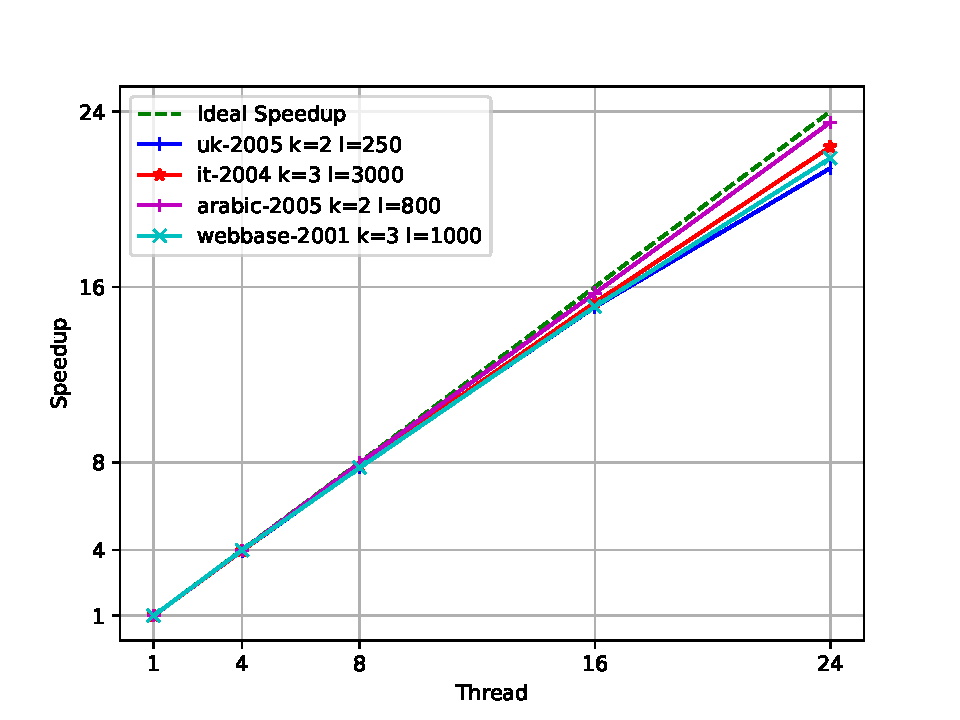
\includegraphics[width=\linewidth]{pic/parallel.pdf}\\
            \caption{The speedup of ListPlex for the large graphs with different parameters. }
          \end{figure}
    \end{minipage}
\end{frame}
\begin{frame}{Excluding unfruitful seed sets}
    \begin{figure}[htb]
        \centering
        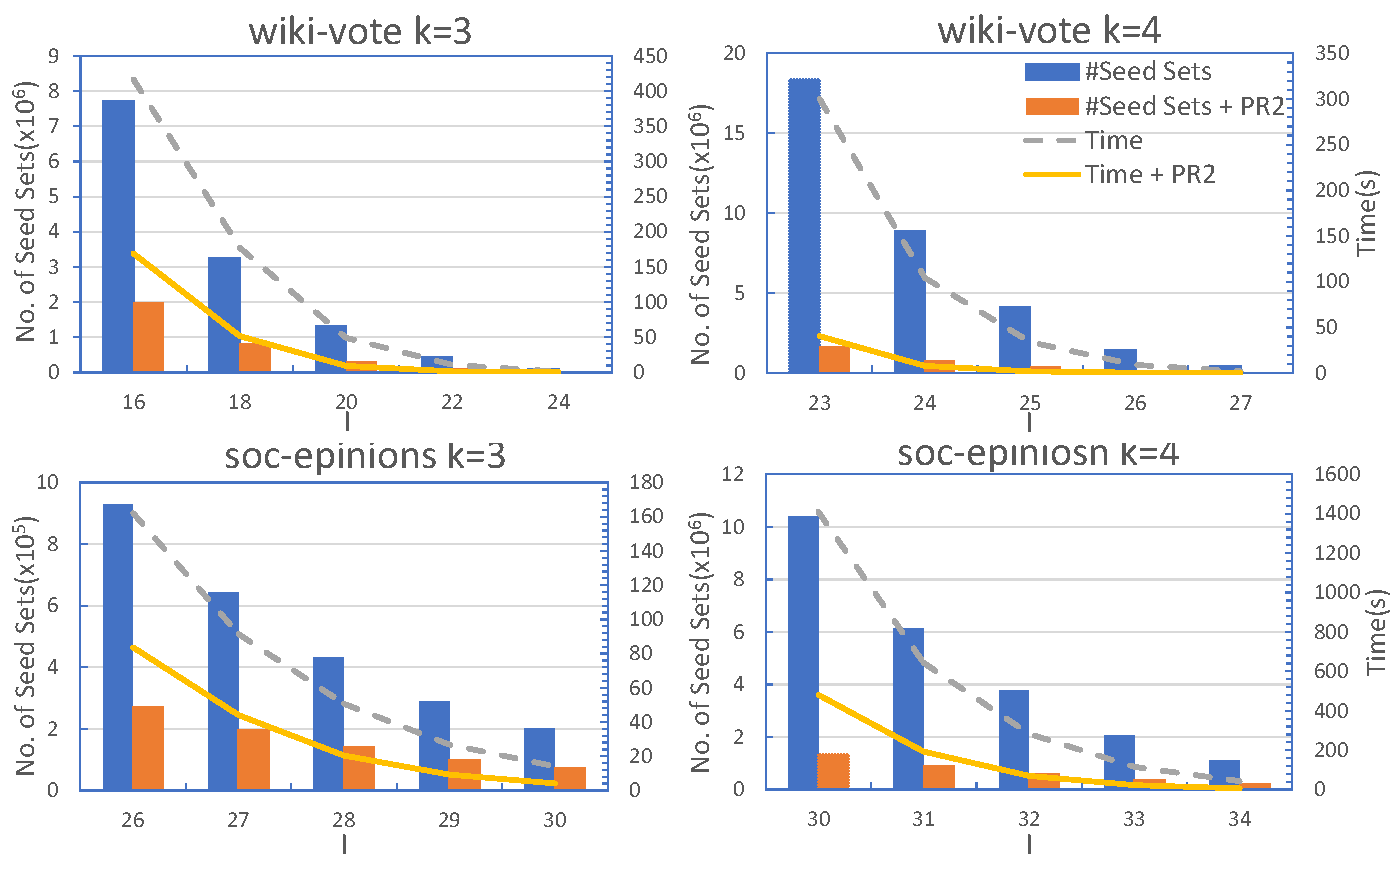
\includegraphics[width=0.8\linewidth]{pic/prune.pdf}
        \caption{The number of seed sets and running time with and without Prune Rule 2.}
      \end{figure} 
\end{frame}
\begin{frame}{Reducing cache misses}
    \begin{figure}[htb]
        \centering
        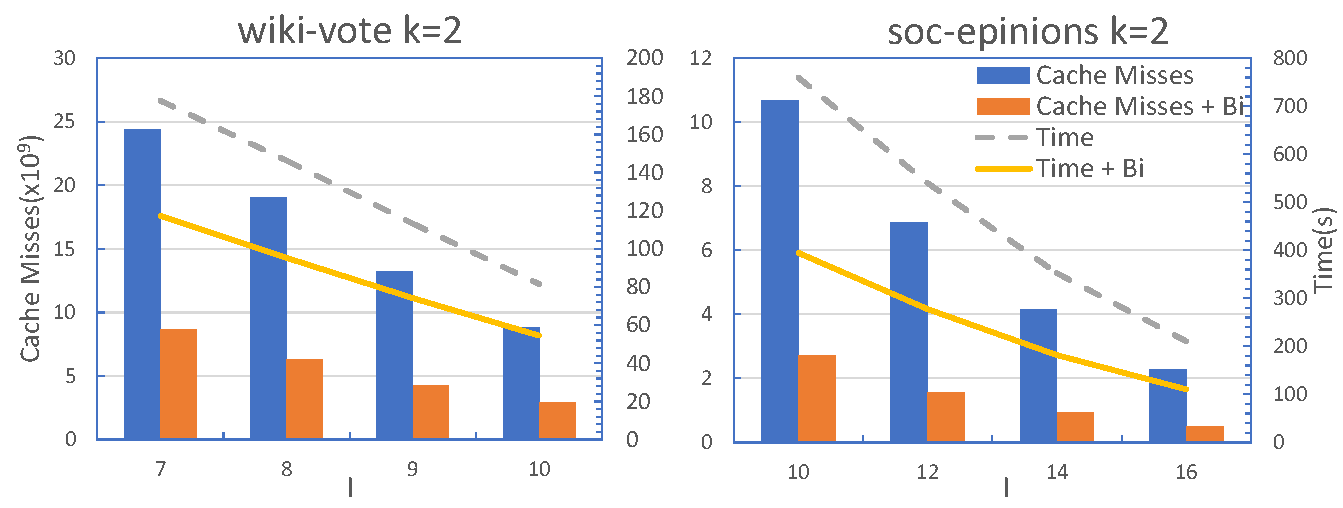
\includegraphics[width=0.8\linewidth]{pic/bipartite.pdf}\\
        \caption{The total number of data cache misses and the running time with and without using bipartite graph $B_i$.}
    \end{figure}
\end{frame}
% \section{Further Discussion}
% \begin{frame}{Ordering}
%     The power of ordering has been discussed for a long time.\\
%     \vspace{0.5cm}
%     Q: Is there a better ordering?\\
%     \begin{itemize}
%         \item Repeatedly removing a node $v$ which minimizes $|N(v)|$ and tie-breaking on $|N^2(v)|$ in the remaining graph?
%         \item Repeatedly removing a node $v$ which minimizes $|N(v)|+|N^2(v)|$ in the remaining graph ($2$-club)?
%     \end{itemize}
% \end{frame}
% \begin{frame}{Branch Scheme}
%     For the worst-case time complexity, the below theorem holds.
%     \begin{theorem}\label{Thm:R-time}
%         Given a graph $G$ with degeneracy $D$, ListPlex runs in $O^*(\gamma_k^D)$ for fixed $k$, where $\gamma_k<2$ is the largest root of $1=x^{-1}+\dots+x^{-k-1}$.
%     \end{theorem}
%     When $k$ = 1, 2, 3, 4, and 5, $\gamma_k$= 1.618, 1.839, 1.928, 1.966 and 1.984, respectively.\\
%     \vspace{0.5cm}
%     Q: Is there a better branch scheme satisfying the following conditions?
%     \begin{itemize}
%         \item Listing $1$-plexes runs in $O^*(3^{\frac{n}{3}})$ time\footnotemark[6],
%         \item Listing $2$-plexes runs in no more than $O^*(X)$ time\footnotemark[7].
%     \end{itemize}
%     \footnotetext[6]{Tomita et al. (2006)}
%     \footnotetext[7]{XXX et al. (20XX)}
% \end{frame}

\begin{frame}
    \begin{center}
        {\Huge Q\&A}
    \end{center}
\end{frame}
\begin{frame}
    \begin{center}
        {\Huge Thanks!}
    \end{center}
\end{frame}

% \section{Appendix}
% \begin{frame}{Experiment Setup}
%     \begin{itemize}
%         \item C++11 and g++-9.3.0 with '-O3',
%         \item The OpenMP shared-memory library,
%         \item Ubuntu20.04 OS, two-way Intel Xeon Gold 6130 CPUs (2.1GHz, 22MB L3-cache, 2 CPU chips and 32 physical cores in total), a 132G RAM and a 1T SSD,
%         \item Hyper-threading and turbo techniques disabled.
%     \end{itemize}
% \end{frame}
\end{document}